\documentclass{article}
\usepackage{FinalYearProjectReport}

% packages for references
\usepackage{cite}
\usepackage{url}


% uncomment this line to double line spacing for proof reading
% \linespread{2}

% packages and settings for graphics
\usepackage[pdftex]{graphicx}
\graphicspath{{./}}
\DeclareGraphicsExtensions{.png}
\usepackage[final]{pdfpages}


\title{Traffic Reporter - Final Report}
\name{Mike Little}
\address{Department of Electrical and Computer Engineering\\
University of Auckland, Auckland, New Zealand}


\hyphenation{and-roid}


\begin{document}

\begin{titlepage}


\vspace*{15em}


\centering

{\LARGE
Department of Electrical \& Computer Engineering \\
Final Year Research Project 2013, Final Report}

\hspace{2em}

% notes on latex tables use "&" as colum sperator
\begin{table*}[h]
\centering
\begin{tabular}{ll}
Project Title: & Traffic Information Engine for Auckland Traffic Lights \\
Project Number: & 14 \\
Supervisor Name: & Dr. Nasser Giacaman \\
Second Examiner Name: & Dr. Partha Roop \\
Your Name: & Mike Little \\
Your UID: & 2626904 \\
Partner Name: & Andrew Luey \\
Date submitted: & 15 September 2013 \\

\end{tabular}
\end{table*}
\begin{table}


\end{table}
\pagebreak

\vspace*{25em}

{\Large Declaration of Originality}

\hspace{5em}

This report is my own unaided work and was not copied from 
nor written in collaboration with any other person.

Name: Mike Little


\end{titlepage}




\maketitle

\begin{abstract}

\end{abstract}

\section{Introduction}
\subsection{Objective}
Auckland Transport has an application that they use to view and analyse traffic volume. The application was last updated in 2007 and is lacking in features and usability. My partner and I were tasked with recreating this application using modern technologies with the goal of improving the features already existing in the application, and adding new features.

\subsection{Motivation}
According to the 2006 census, travel by car accounted for 48\% of travel and 44\% of travel was by public transport. Up to 2030 60\% of New Zealand's population growth is going to occur in Auckland. In terms of numbers of trips, in 2006 there were approximately 4 million trips per day in Auckland. This number is projected to grow to 5.5 million trips per day in 2041.

There is limited ability for Auckland to expand its road network so Auckland transport should focus on making their current road infrastructure more effective. A better understanding of Auckland's traffic would lead to better city planning and traffic optimization.

\subsection{Background}

At an intersection with traffic lights, under each lane there are inductive loops that can detect when a vehicle travels over them. Every 5 minutes these detectors send their counts to that intersection's traffic controller. The traffic controller sends the volume data to Auckland's SCATS server \cite{sims1981scat}. See Figure \ref{fig:background}. 

\begin{figure}[!t]
\centerline{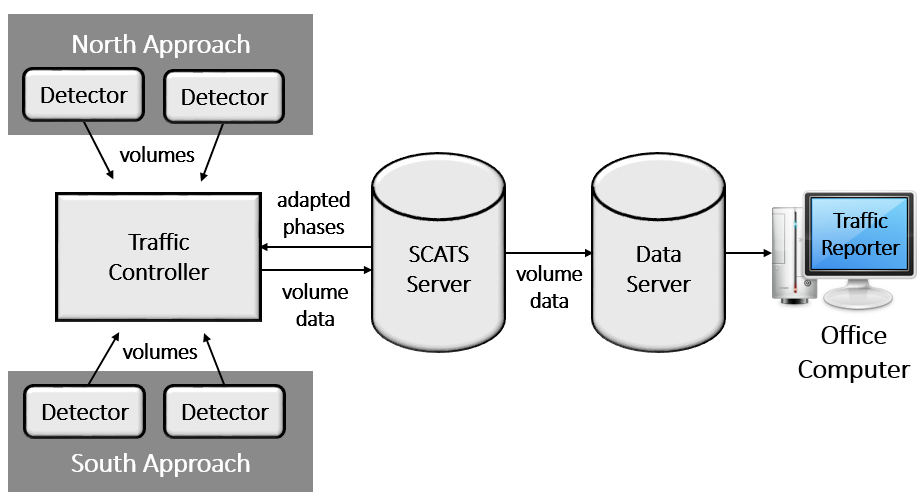
\includegraphics[height=1.8in]{background}}
\caption{Flow diagram of a single intersection}
\label{fig:background}
\end{figure}

The SCATS server can use this volume data to adjust traffic light phases to suit the traffic trends. For example if there is a large volume of traffic headed towards the city centre at a certain intersection, the next intersection will have longer green phases for cars travelling in that direction. While SCATS does lag behind actual traffic trends by 5 minutes, automatically adjusted traffic phases have been shown to be more efficient than statically phased intersections.

As well as adjusting the traffic light phases, the SCATS server also saves the volume data to a data server where it is available for later viewing and analysis in binary *.vs files. Auckland Transport's traffic engineers use an application called Traffic Reporter which can open these files and view the data in a table or graph view.


\section{Requirements}
\subsection{Requirements Gathering}
For this project we have had weekly or fortnightly
meetings with our client. To begin with these meetings were
used to gather requirements and to find out more about how
the existing application works and what it is used for.
The main use of the existing application is to use the
volume data for reports. For example, finding the busiest
intersections for a given month, or finding the busiest time of
day for different intersections, etc.

We also went to the Auckland Transport office in the
Auckland CBD. We saw that it is used in tandem with another
program that directly interfaces with SCATS. The other
program shows detectors being triggered in pseudo real time
and shows planned and actual light phasing. Also available to
them were camera feeds of some of the main intersections.
Using all of these tools they could identify an intersection
whose phasing is incorrect or non-optimal and then check the
volumes of those intersections to see if there are any obviously
faulty detectors.

The visit to Auckland Transport was instrumental in our
understanding of what it is we are trying to replicate and
improve. We were able to identify significantly more use
cases, from seeing the application in action in the environment
that it is used in.

\subsection{Functional Requirements}
From our meetings with our client, we ascertained a number of functional as well as non-functional requirements. The initial functional requirements were as follows:

\begin{itemize}
	\item Recreate table and graph views
	\item Improve upon these views, giving more details.
	\item Add exporting Microsoft Excel
	\item Add the ability to save configurations
\end{itemize}

As the project progressed and time and scope allowed for more features we were given more requirements:

\begin{itemize}
	\item Be able to find suspected faulty detectors
	\item Produce a report over multiple days, giving statistics for each day and averages
\end{itemize}

\subsection{Non-Functional Requirements}

In our initial meetings there was a big focus on when recreating the application to make it extensible, so that after we had finished the project could be picked up by someone else and continue to work on with little effort.

One of the complaints about the original Traffic Reporter is that it is lacking in aesthetics and usability. One of our client's intentions in having the program recreated was to make it more usable and bring it up to modern standards. 

\section{Research}
\subsection{Existing Application}
To recreate the existing application, we had to become
familiar with it. We explored its features and what we liked
and disliked about it.

The current application has two modes; essentially it is two
programs in one. One mode displays information on traffic
volume (the VS mode), the other displays information on the
traffic light phasing. Because of scope constraints we looked
only into the traffic volume part of the application. 

The VS mode has four different views; a graph view, a
table view, a column view, and a dump view. The two most
commonly used views are the graph and table view. We were
unable to ascertain what the column view is actually used for.
The dump view gives a human readable representation of a
volume store file that is very close to how it is encoded. This
was useful to us when we were learning how to read the files,
but is unused otherwise.

The graph view (See Figure \ref{fig:oldGraph}) shows a line graph with time on the X-axis
and traffic volume on the Y-axis. Each detector at an
intersection can have its own series or they can be grouped
together. The time interval can be set between 5 minutes and
an hour. Data is collected every 5 minutes, so if you increase
the interval it plots the average.

\begin{figure}[!t]
\centerline{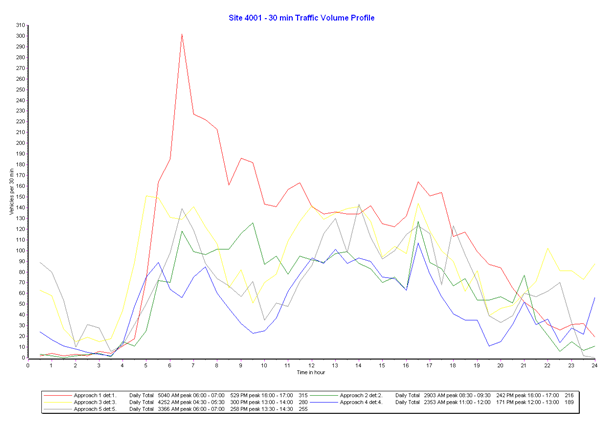
\includegraphics[height=2.3in]{oldGraph}}
\caption{Screenshot of the graph view from the original Traffic Reporter}
\label{fig:oldGraph}
\end{figure}

The graph view is useful for seeing trends in traffic flow.
For example for some detectors there is a large spike between
6am and 7am and then it falls off over the rest of the day. We
can look at this and see that that detector probably heads
toward the CBD.

\begin{figure}[!b]
\centerline{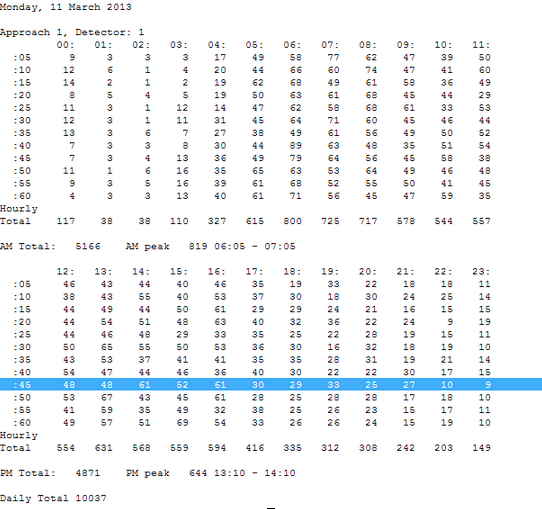
\includegraphics[height=2.3in]{oldTable}}
\caption{Screenshot of the table view from the original Traffic Reporter}
\label{fig:oldTable}
\end{figure}

The table view displays volume information for 5-minute
intervals for each hour with hourly totals in the bottom row
(See Figure \ref{fig:oldTable}). There is a table for both AM and PM traffic with
the total for each half of the day and the peak amount and
time. Each approach has its own pair of tables, so like the
graph view you can group detectors together to get an
indication of volume for a specific direction. You can change
the interval to get the totals over that interval.
The table view is good for finding specific values at
specific times, but is poor for identifying trends.
The column view is used only to export data to an Excel
spreadsheet for further manipulation.

\begin{figure}[!t]
\centerline{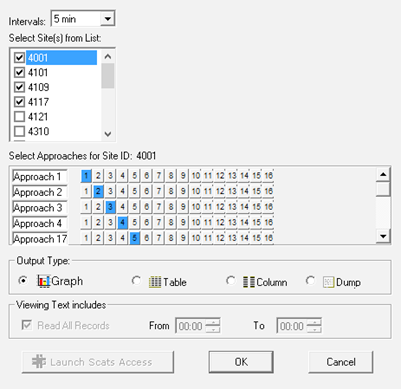
\includegraphics[height=2.3in]{oldConfig}}
\caption{Screenshot of the configuration screen from the original Traffic Reporter}
\label{fig:oldConfig}
\end{figure}

To select what intersection is displayed in any of these views you use the configuration screen, which is essentially a wizard that displays when the application starts after loading a volume file (See Figure \ref{fig:oldConfig}). To select the intersection is confusing, as it combines both a list item selection and check boxes. Once you have selected an intersection you can group detectors into approaches using a table of radio buttons. Also the window for the wizard cannot be resized, so you're limited to viewing only 5 approaches at a time.


\subsection{Potential Solutions}
One of the requirements that the client stressed to us was
future extensibility of platforms. To make the application
portable we initially suggested making a web based
application with a RESTful API \cite{fielding2002principled}. This way it would be
very easy to introduce new platforms that would only have to
make use of the API.

The other choice was a windows desktop application that
loads volume files locally. The main advantage of this
platform choice would be that there would be significantly less
architectural work involved and could be developed more
rapidly.

Due to time constraints and infrastructure requirements, with our client we decided to implement a Windows application.
In creating this we had a number of options available to us; but the two most promising were to write the application using Java and the Swing GUI Framework \cite{swing} or C\# with the Windows Presentation Foundation (WPF) \cite{wpf}.

We were more familiar with Java and Swing but we thought that as we were creating a Windows application, why not use a language and framework tailor made to making one? Also WPF has some very interesting data binding capabilities that we wanted to investigate, so we chose to use that combination.

In the original Traffic Reporter asks you to import volume data files each time you run the application. We initially took this approach, but found that loading these files each time became annoying as it took at least 30 seconds per file. So we decided to have a one time import into a database. We chose SQLite \cite{sqlite} as we thought that the scale of our application was appropriate for a file based database rather than a server based one.

\section{Traffic Reporter 2013}

\subsection{Overview}

In Figure \ref{fig:overview} we can see a screenshot of Traffic Reporter 2013. At the top we have the Toolbar which lets you switch between the various modes of the application. 

We have four different modes; the Home mode, which lets you view the days for which you have imported data, the Summary mode that lets you view average statistics for multiple days, the Reports mode which lets you view tables and graphs like the original application, and the Faults mode which lets you view detectors which are suspected to be faulty.

On the left is the Report Browser which is used by both the Summary Mode and the Reports Mode. It lets you select the displayed report or summary and create new ones.

\begin{figure}[!h]
\centerline{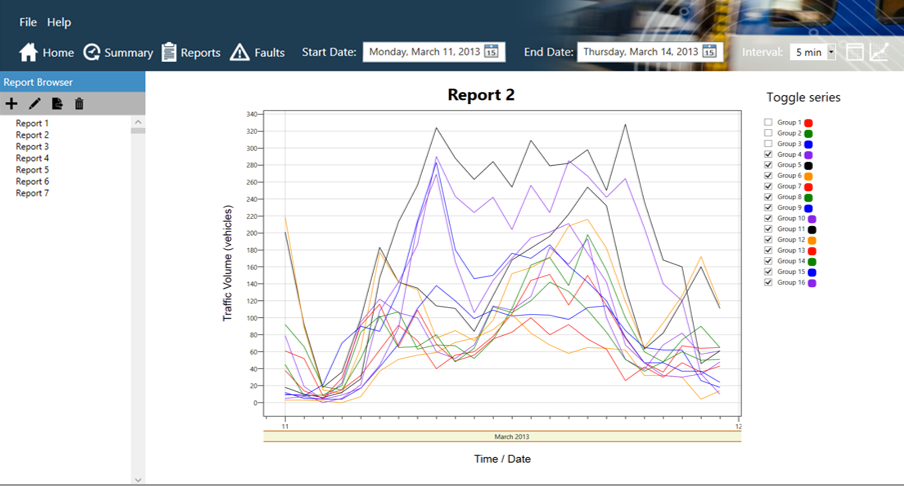
\includegraphics[width=3.1in]{overview}}
\caption{Screenshot of the configuration screen from Traffic Reporter 2013}
\label{fig:overview}
\end{figure}

\subsection{Improved Features}
In Traffic Reporter 2013 there were a number of features from the original application that we thought we could improve on. This section details the improvements and changes we made per feature in the original application.

\subsubsection{Configuration Screen}
In the configuration screen we really wanted to improve on the usability and efficiency. In the original application the configuration screen uses a table of radio buttons to group detectors. The window cannot be resized so you can only view 5 approaches at a time. In our screen (See Figure \ref{fig:newConfig}) there is a lot more space available and we use a drag and drop interface to group detectors into approaches. 

\begin{figure}[!t]
\centerline{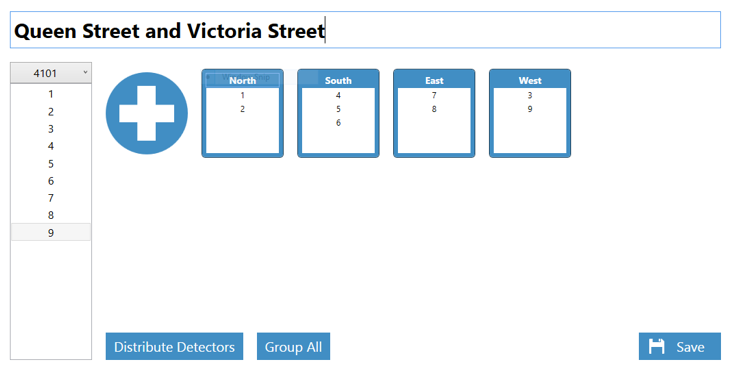
\includegraphics[width=3.1in]{newConfig}}
\caption{Screenshot of the configuration screen from Traffic Reporter 2013}
\label{fig:newConfig}
\end{figure}

At the top you can enter the name of your configuration. To the left is a drop-down box which will list the intersections you have volume data imported for. When you select an intersection the list view below is populated with the detectors for that intersection. From that list view you can select multiple detectors and drop them either onto the plus sign to create a new approach control, or onto an existing approach control. Each approach control has a name and detectors can be dragged and dropped between them. The approach control was a custom control we created for the configuration screen. Dragging and dropping multiple detectors at a time is much more intuitive and efficient than the interface in the old Traffic Reporter.

At the bottom left of the screen are two buttons for convenience. The button titled ``Group All'' puts all detectors into a single approach named ``All Detectors''. The button titled ``Distribute Detectors'' puts each detector into its own Approach named ``Group *'' (where * is the number of the detector). These buttons were one of the major improvements over the previous version of Traffic Reporter because traffic engineers would often waste time with the table of buttons based interface grouping detectors in these ways.

\subsubsection{Table View}
In the table view of the original Traffic Reporter the data was represented by two ASCII tables per approach, one each for AM and PM. With each table were additional statistics; the total traffic volume, the peak volume and period. 

To improve upon this we created a view (See Figure \ref{fig:newTable}) that used a data grid control and added an overview of statistics over all approaches. Given that we had more screen space we also combined the AM and PM tables into one table spanning 24 hours.
The overview statistics lists the busiest approach with the corresponding volume count, the busiest AM and PM periods of all the approaches and their volume counts.

\begin{figure}[!t]
\centerline{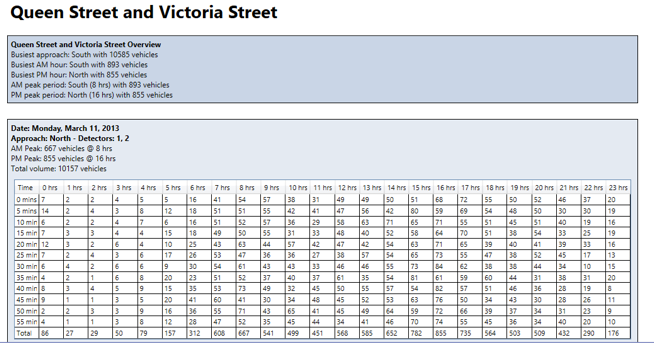
\includegraphics[width=3.1in]{newTable}}
\caption{Screenshot of the table view from Traffic Reporter 2013}
\label{fig:newTable}
\end{figure}

\subsubsection{Graph View}
In the new graph view there are a few small improvements over the original. In the original some of the colours used for the series didn't contrast enough against the white background, and so were difficult to see. We limited the set of colours for series to colours that contrasted against white. We also added added the ability to toggle different series on the graph. When a series is hidden the graph resizes its axes for an optimal fit. Error values for faulty detectors are represented by the number 2047, so significantly dwarf other values. Toggling series with errors in them allows the other series to be viewed more easily.

\begin{figure}[!b]
\centerline{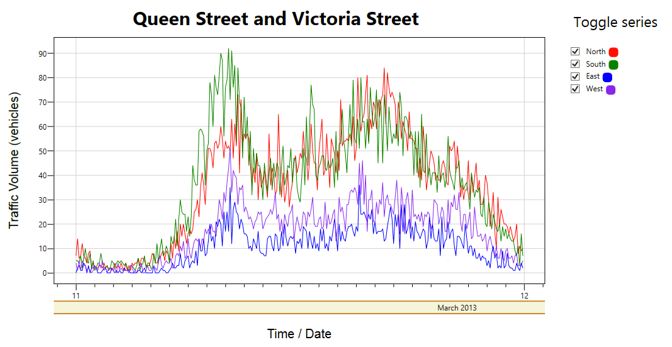
\includegraphics[width=3.1in]{newGraph}}
\caption{Screenshot of the graph view from Traffic Reporter 2013}
\label{fig:newGraph}
\end{figure}

\subsubsection{Importing Files}
In the original application you would have to specify the file you want to read from (A single file contains a data for 24 hours). We went with this approach to begin with, but found that reading the same file every time we ran the application was time wasted. We decided that we would do a one time import into a database.

To import the files into the database and store meaningful values we needed to decode the binary data in the files (See Figure \ref{fig:vsDataFormat} for data format). From the decoded data we insert each volume count as a row into the volumes table with a datetime, intersection, detector number and corresponding volume. The datetime, intersection and detector number can uniquely identify a volume count.

\begin{figure}[!t]
\centerline{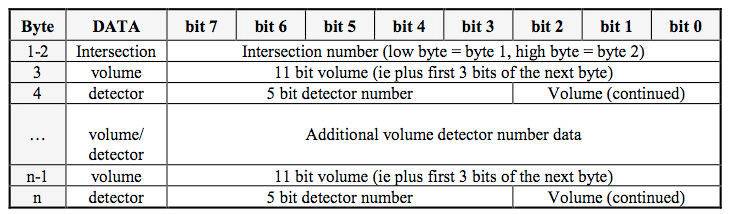
\includegraphics[width=3.1in]{volumeDataFormat}}
\caption{Format of a volume record in a *.vs file}
\label{fig:vsDataFormat}
\end{figure}

When importing some data files, we found that they sometimes contained duplicate data. This caused errors because key constraints were being violated. This was indistinguishable from when the user tried to import the same file twice and we needed some way for the user to indicate what should happen in case of a duplicate. 

As such whenever this occurs, by default the user is asked if they wish to skip this file, skip all files (Traffic Reporter 2013 can do batch importing), or continue processing the file. There is a user setting that lets you set the default option, skip, continue, or ask every time. Specifying a default option lets the user leave the application importing a large amount of files overnight, which is important because one file can take upwards of a minute to be processed, longer if there are duplicates.

\subsection{New Features}

In addition to improving existing features, we also added a few new features with the intention of increasing the efficiency of Auckland Transport's traffic engineer's workflows.

\subsubsection{Suspected Faults}

\begin{figure}[!b]
\centerline{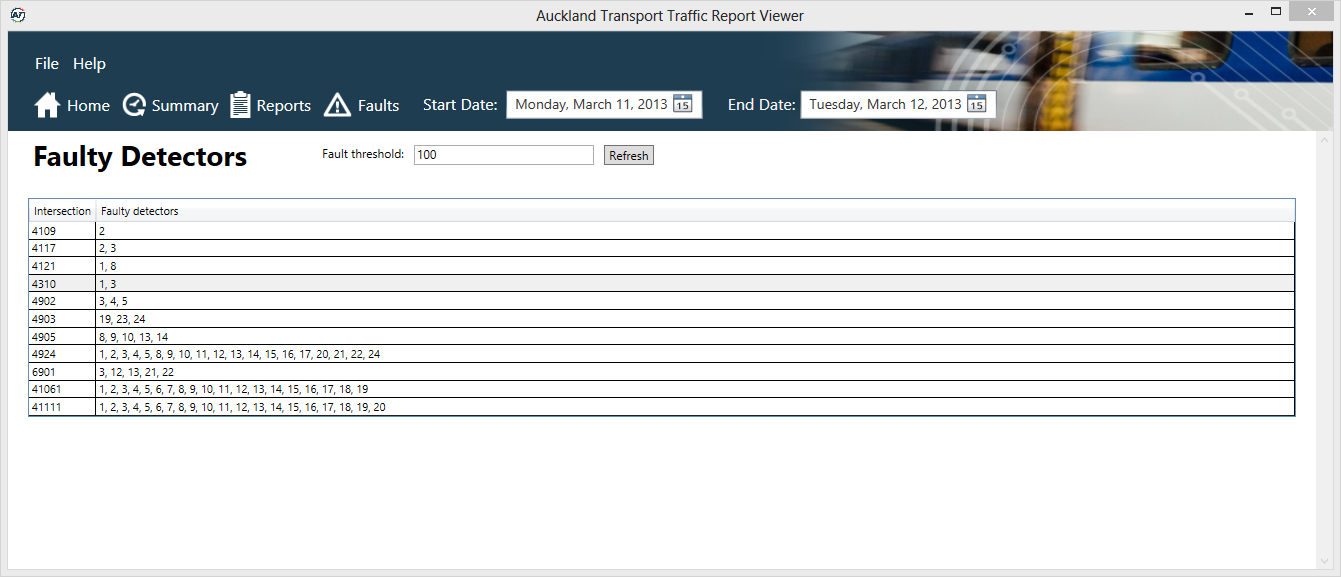
\includegraphics[width=3.1in]{faults}}
\caption{View of Faults Screen}
\label{fig:faults}
\end{figure}

Currently Auckland Transport relies on angry motorists calling and telling them that an intersection isn't phasing correctly. SCATS has no way of indicating that a detector may be faulty or not.

The Faults mode (See Figure \ref{fig:faults}) lists all of the detectors grouped by intersection that have volume over the threshold in the date range specified in the Toolbar. The threshold defaults to 100 (the theoretical maximum volume in a 5 minute period) but can be changed.

\subsubsection{Summaries}
One of the ways the original application was used was to copy data from the table or column view and paste it into Microsoft Excel for further calculations and analysis. One of the common calculations was the average of certain stats over a month. The intention of the summary mode is to bring some of the calculations into Traffic Reporter to remove the tedious and time consuming task of copying and pasting statistics one day at a time.

In Summary mode we have three calculated statistics; daily total volume, AM peak hour total volume, PM peak hour total volume. These are displayed per day per route.

A route is a collection of detectors for an inbound and outbound intersection. These routes are specified using the summary configuration screen (See Figure \ref{fig:summaryConfig}).

The summary configuration screen lets you specify routes using a DataGrid, entering data into a row in the table will create another empty row below it, letting you create a summary with multiple routes. The inbound and outbound dividing factors are used for when summaries are exported in a CSV format.

\begin{figure}[!b]
\centerline{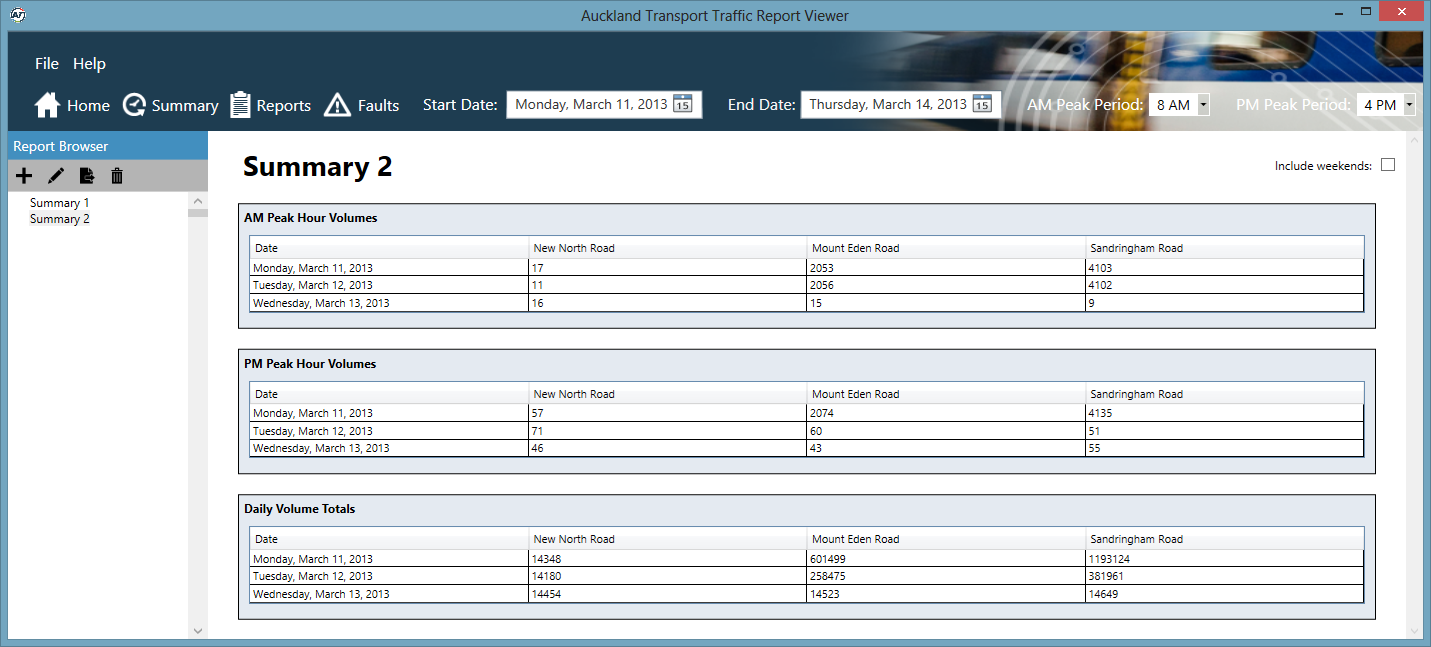
\includegraphics[width=3.1in]{summary}}
\caption{Screenshot of the summary mode from Traffic Reporter 2013}
\label{fig:summary}
\end{figure}

\begin{figure}[!b]
\centerline{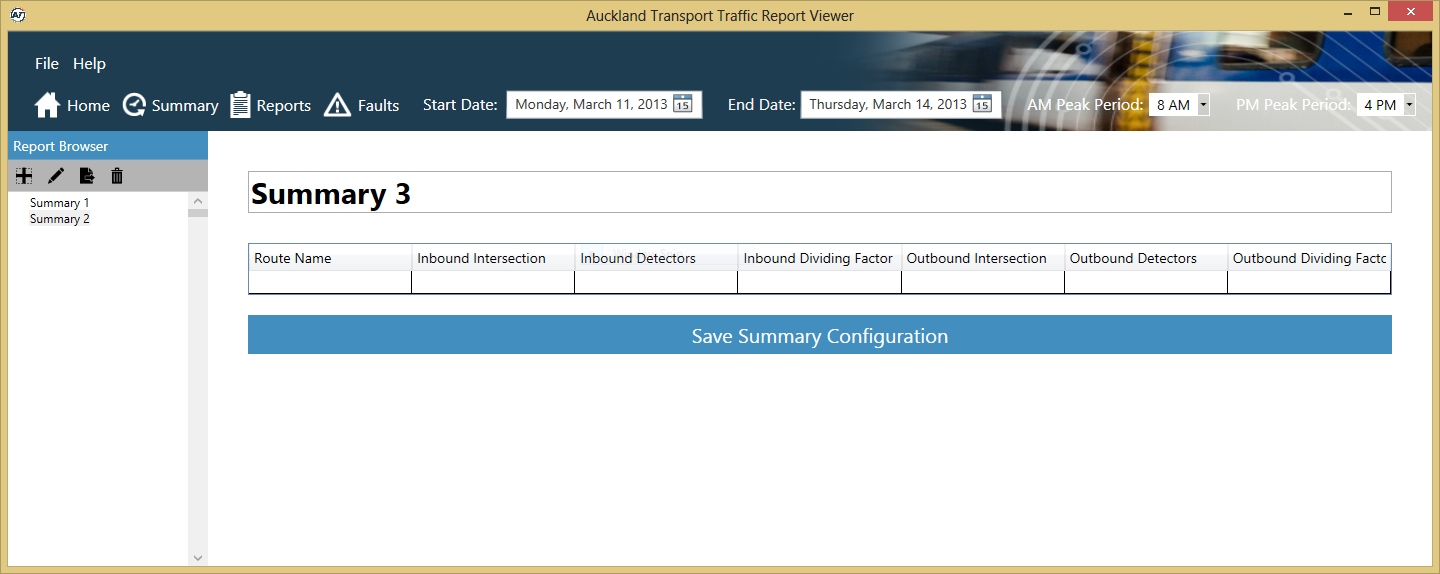
\includegraphics[width=3.1in]{summaryConfig}}
\caption{Screenshot of the summary configuration screen from Traffic Reporter 2013}
\label{fig:summaryConfig}
\end{figure}

\subsubsection{CSV Exporting}
While we were able to bring some analysis back into Traffic Reporter, we knew that it would be tedious to bring all that functionality into the application. We wanted it to be easy to do further analysis in Excel so we added the ability to easily export to a CSV format. We added this ability for summaries and reports. 

An exported report has the same layout as the table view in the application. An exported summary is not exactly identical to what you would see on a summary view, it also includes the configuration table which has the inbound and outbound dividing factors (See Figure \ref{fig:summaryCSV}).

Exporting to CSV lets traffic engineers have the workflow of doing further analysis in Excel without the tediousness of copying and pasting individual days' statistics. 

\begin{figure}[!t]
\centerline{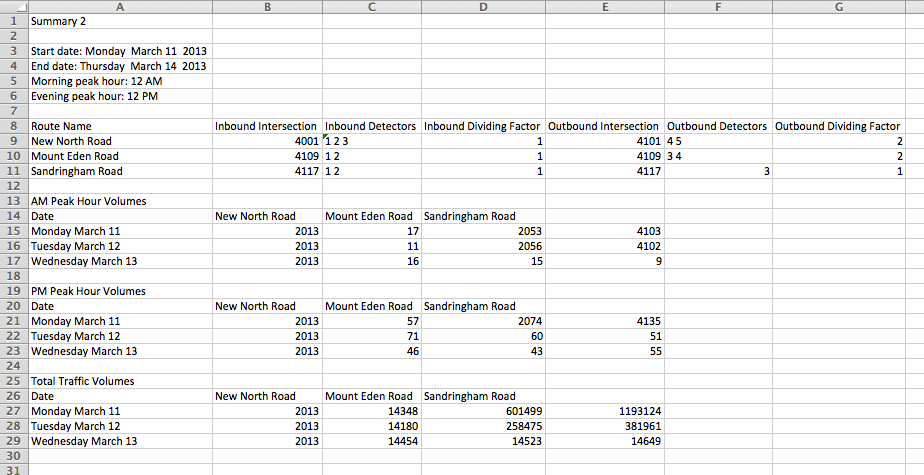
\includegraphics[width=3.1in]{summaryCSV}}
\caption{Screenshot of exported summary}
\label{fig:summaryCSV}
\end{figure}

\section{Architecture}
Our architecture can be described as comprising of two essential parts; a data source, and presentation logic. See Figure \ref{fig:architecture} for a view of Traffic Reporter 2013's architecture.

\begin{figure}[!b]
\centerline{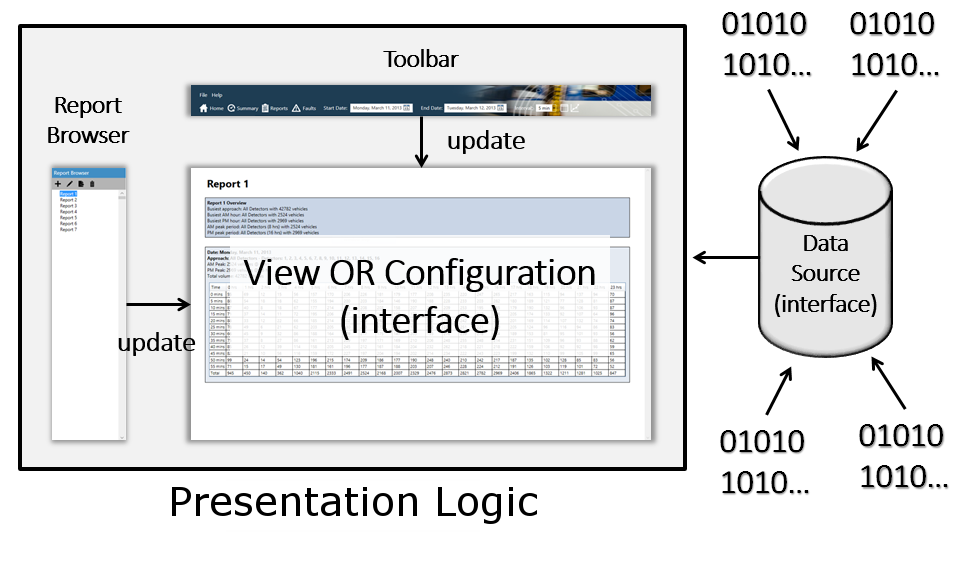
\includegraphics[width=3.1in]{architecture}}
\caption{View of application architecture}
\label{fig:architecture}
\end{figure}

\subsection{Data Sources}
Because there was a major focus on extensibility from our client and we originally wanted to create a web service, we abstracted the way our application gets its volume data and configurations. We do this using an interface appropriately called DataSource. This interface has methods for retrieving volume counts for a detector at a datetime, getting a list of intersections, getting a configuration by its name, etc. In our application we created an implementation of this interface that communicates with an SQLite database.

If we later wanted to switch to retrieving data from a web service we could write an implementation that sends HTTP requests to the server and then constructs objects the presentation logic understands from the JSON response.

If we wanted to change the backing database from SQLite to SQL Server we could write an implementation that connects that does connects and executes SQL queries for that.

\subsection{Presentation Logic}
In our presentation logic there are 3 main components; the Toolbar, the Report Browser, and the content screen. The content screen  is a WPF UserControl that implements either the ViewScreen or ConfigurationScreen interfaces. 

These interfaces allow the screen to respond to and emit events that are sent and consumed by the Toolbar and Report Browser. For example, in the ViewScreen interface there is an event handler to respond to the date range being changed in the Toolbar. There is also an event handler declared to let a ViewScreen know when the selected report in the report browser changes.

The ConfigurationScreen interface declares an event that lets the screen tell the rest of the application that a new configuration has been created and saved. This event is consumed by the report browser which can update its list of reports.

The Report Browser and Toolbar are custom controls that are all contained by a MainWindow control that connects all the event and event handlers. The MainWindow also subscribes to some of the events from the Toolbar and Report Browser and emits events itself and is responsible for switching screens and giving the user access to application settings.

\section{Reflections}
In reflection there are some things that we would have done differently in the development of our solution and some things that we thought went very well.

Our choice of using SQLite as our backing DataSource was perhaps not the best. We initially thought that the scale of our application would best be suited by a small database like SQLite. However, as we started having more complicated queries and requesting larger amounts of data more frequently we started seeing performance issues. 

We thought that we could offload the database fetches to a worker thread to keep the UI reactive, but multiple threads and a file based database resulted in the database being locked every so often. 

A more suitable replacement could be SQL Server, as it would integrate well with C\# and WPF, all of them being Microsoft products.

Something we thought we did well was our development process and division of work. There weren't many times when my partner and I were blocked waiting on each other to complete something. We were able to break down the tasks so that there was always something that could be done instead of waiting. 

When we did work together it was when we needed to make a key architectural or directional decision, or when one of us was finding a task difficult and needed a new perspective on the problem.

Another element that was key to the success of our project, was our customer collaboration. Having regular feedback from an actual user of the original application let us know when we were actually creating features and workflows that were an improvement. Meeting every two weeks gave us time to do substantial work, but was short enough that we did not progress significantly in a bad direction.

\section{Conclusions}

In conclusion, we were tasked with recreating the Traffic Reporter application using modern technologies with the goal of improving the features already existing in the application, and adding new features. 

We created a standalone Windows application using C\# and the Windows Presentation Foundation. We replicated and improved upon the original Traffic Reporter's features and introduced some new features that will improve the effectiveness and efficiency of Auckland Transport's traffic engineers.

Through customer collaboration and effective development processes we were able to create an application that we believe more than improves upon the original Traffic Reporter.

\section{Future Work}

In the future we would like to port the backing data source to a web service. This was our intial proposal that we thought would satisfy the extensibility non-functional requirement.

More work can be done to have more intelligent fault detection. Currenly the fault detection only will find detectors with suspiciosly high volume counts. There are also situations where a faulty detector will report zero volume, the current logic will not detect these faults.

We would liked to have indications in the two report views that a volume count could be faulty. In the table view we would have highlighted suspicious cells, in the graph view we would put a red dot where the point was suspicious.

We would have liked to add the feature of exporting configurations so that traffic engineers could shared them instead of having to construct them each themselves.

\bibliographystyle{IEEEtran}
\bibliography{final_report}


\end{document}